\documentclass[11pt]{article}

\usepackage{amsmath}
\usepackage{amsthm}
\usepackage{amsfonts}
\usepackage{amssymb}
\usepackage{mathrsfs}
\usepackage{hyperref}
\usepackage{listings}
\usepackage{graphicx}
\usepackage{xcolor}

\definecolor{codegreen}{rgb}{0,0.6,0}
\definecolor{codegray}{rgb}{0.5,0.5,0.5}
\definecolor{codepurple}{rgb}{0.58,0,0.82}
\definecolor{backcolour}{rgb}{0.95,0.95,0.92}
 
\lstdefinestyle{mystyle}{
    backgroundcolor=\color{backcolour},   
    commentstyle=\color{codegreen},
    keywordstyle=\color{magenta},
    numberstyle=\tiny\color{codegray},
    stringstyle=\color{codepurple},
    basicstyle=\ttfamily\footnotesize,
    breakatwhitespace=false,         
    breaklines=true,                 
    captionpos=b,                    
    keepspaces=true,                 
    numbers=left,                    
    numbersep=5pt,                  
    showspaces=false,                
    showstringspaces=false,
    showtabs=false,                  
    tabsize=2
}
\lstset{style=mystyle}

\hypersetup{
    colorlinks=true,
    linkcolor=blue,
    filecolor=magenta,      
    urlcolor=cyan,
}
\renewcommand{\qedsymbol}{$\blacksquare$}
\def\multiset#1#2{\ensuremath{\left(\kern-.3em\left(\genfrac{}{}{0pt}{}{#1}{#2}\right)\kern-.3em\right)}}

\newtheorem{theorem}{Theorem}
\newtheorem{lemma}{Lemma}
\newtheorem{corollary}{Corollary}
\newtheorem*{definition}{Definition}
\newtheorem*{example}{Example}
\newtheorem*{note}{Note}
\newtheorem{exercise}{Exercise}
\newcommand{\bproof}{\bigskip {\bf Proof. }}
\newcommand{\eproof}{\hfill\qedsymbol}

\usepackage[a4paper,margin=1in,footskip=0.25in]{geometry}
% \setlength\parindent{0pt}

\title{Euclidean Minimum Spanning Tree in Low Dimensions}
\author{An Nguyen (aqn180001@utdallas.edu)}

\begin{document}
\maketitle

\begin{abstract}
	Euclidean Minimum Spanning Tree has many applications, particularly as a heuristic for search problems or clustering algorithms. We compiled and implemented three fast EMST algorithms based on Prim's, Kruskal's, and Boruvka's MST algorithms for undirected graphs. Our tests on synthetic data shows that Bentley Friedman's algorithm works especially well on low dimesional data and that the state of the art GeoMST and Dual Boruvka's algorithm remains scalable, but works slow without a well written space partitioning tree.
\end{abstract}

\section{Introduction}

The  Euclidean  Minimum  Spanning  Tree  problem  involves  finding  the  smallest  cost  (in  euclidean distance) MST for a point set in $\mathbb{R}^d$. Most MST algorithms are based on Tarjan's two rules: the cut / blue rule and the cycle / red rule. They denote different properties of the minimum spanning tree.

\textbf{Blue Rule}. This rule states that the minimum edge accross any cut belongs to a MST. A cut is defined as a partition of the graph into two sets of vertices. 

\textbf{Red Rule}. This rule states that for any cycle, the heaviest weight edge cannot be in the MST.

A vast majority of MST algorithms focuses on using the blue rule to iteratively construct the MST. Kruskal's algorithm and Prim's algorithm, for example, use this idea and achieve a complexity of $O(m\log{n})$ and $O(m + n\log{n})$ respectively. However, as there are $O(n^2)$ edges in an instance of the Euclidean Minimum Spanning Tree problem, these approaches warrants further optimization. 

\subsection{Bentley and Friedman}

In 1977, Bentley and Friedman introduced an approach for the Euclidean Minimum Spanning Tree problem based lousely on Prim's algorithm.\cite{Friedman} The algorithm repeatedly find the minimum weighted edge outgoing from a component of the partially built MST graph, which they called a fragment. One can see that this edge addition follows the blue rule and, if applied repeatedly, constructs a MST on the original graph. 

To find the nearest neighbor (minimum edge) of a fragment, they utilize a kd tree. A kd tree is a space paritioning tree which maintains a point set. Each node corresponds to a subset of the points. Any inner node splits its subset of points using a hyperplane intersecting one of the points, which divides the space into two parts. Points that belong to the ``left" part belongs to the left child of the node, and points the belong to the ``right" space belongs to the right child.

One can find the nearest neighbor in the point set of a point $p$ by a pruned depth first traversal of the tree. The traversal visits the subtree whose bounding box is closest to $p$, and will prune a node if the distance between $p$ and the bounding box of that node is at least the closest distance observed so far in the traversal. Though there is no strict bounds, if the k-d tree is balanced then the nearest neighbor queries is observed to be $O(\log{n})$.

In this project, we implement a variant of Bentley Friedman which deviates from Prim's algorithm. Instead of growing one fragment into an MST, we grow multiple fragments, giving up on a fragment when the average number of nearest neighbor queries needed to find the minimum weighted edge to a non fragment exceeds some threshold $m_1$.

\subsection{GeoMST - Well Separated Pair Decomposition}

It is well known that the EMST problem and the Well Separated Pair Decomposition problem are closely related. A WSPD of $P$ is a set $\{(A_0, B_0), (A_1, B_1), \ldots, (A_{m-1}, B_{m-1})\}$ where $A_i \subseteq P$ and $B_i \subseteq B$ are well separated and every pair $x,y \in P$ is present in exactly one $A_i \times B_i$. A pair of points $A,B$ are well separated if $dist(A, B) \ge \max\{Diam(A), Diam(B)\}$. $Diam(P)$ denotes the diameter of the smallest hypersphere enclosing all points in $P$ centered at the center of $P$'s bounding box. $dist(A,B)$ denotes the distance between the two bounding hyperspheres of $A$ and $B$. 

In 1995, Callahan and Kosaraju introduced a method for computing a WSPD in $O(n\log{n})$ using fair split tree, which is a space partitioning tree much like a k-d tree.\cite{Callahan} Instead of splitting by a hyperplane on an arbitrary node, we split a node by the middle of the longest dimension of the bounding box of its point set. Unlike the conventional version of a k-d tree, a fair split tree stores points only on its leaves, and explicitly maintain the bounding box of each node.

With WSPD of a point set $P$, one can compute the bichromatic closest pair of $A_i, B_i$ for all $i$, which is defined as the closest pair of points $p \in A_i$, $q \in B_i$. If we consider these pairs as edges for our MST in increasing order of distance, and add them into our MST only if $p$ and $q$ are not in the same connected component, we will get a correct MST. This is because, due to the special properties of a well separated pair, when we consider the BCP of $A_i, B_i$, all points in $A_i$, $B_i$ are guaranteed to have already been connected. This idea is almost identical to Kruskal's, and in the worst case where the WSPD are singleton pairs, works in $O(m\log{n})$. However, it can be showed that we can construct a WSPD with only $O(n)$ nodes, bringing the complexity down to $O(n\log{n} + T)$ where $T$ denotes the total time taken to compute the BCP.

Narasimhan and Zachariasen introduced a method of computing BCP from the fair split tree used to compute WSPD, and relaxed the definition of $dist(A,B)$ to minimum distance between the bounding box of $A$ and $B$, which significantly reduces the amount of square root computation of the algorithm. This method, named GeoMST2, was the state of the art EMST algorithm before the Dual Tree Boruvka algorithm emerged.\cite{Narasihman}

\subsection{Dual Tree Boruvka Algorithm}

In 2010, March et. al. introduced another EMST algorithm based on the Boruvka MST algorithm. Unlike Prim's or Kruskal's, the Boruvka algorithm repeatedly find the nearest outgoing edge from every component of the graph and add them into the MST simultaneously.\cite{Dual} This process repeats until there is only one component. Since every pass at least halves the number of connected components, the algorithm terminates in $O(\log{n})$ of these steps.

The brute force version of this algorithm uses $O(m)$ time per pass, but can be significantly sped up using a space partitioning tree to find nearest point to a vertex not connected to it. This takes $O(nT)$ time where $T$ denotes the time for nearest neighbor query into the space partitioning tree. 

March et. al.'s approach utilizes a dual-tree approach. Rather than querying nearest neighbor one by one, we have a space paritioning tree known as the reference tree for the nearest neighbor, and another dual tree known as the query tree that contains the query points. One can imagine a dual depth first traversal simultaneously in both trees that computes the nearest non connected point for each query node. However, this certainly would take $O(n^2) = O(m)$. Like the Bentley Friedman algorithm, we consider a pruning dual depth first traversal of the two trees that visits the most promising node pairs first and prunes off pairs of node in its visit when it is clear that the closest non connected point distance cannot be improved. March et. al. managed to prove that using a Cover Tree, one can achieve a complexity of $O(n)$. However, since we are limited by time we only consider the version that uses a fair split tree.

\section{Implementation}

For implementation, we take on the challenge of not using any external libraries (only c++ std). A lot of the algorithms featured comes from old papers that does not give explicit details on implementation or assumes that you know of related algorithms. We specify these details in case readers want to reproduce our implementation and results or understand details in our code. 

\subsection{Challenges with Bentley Friedman}

The implementation for Bentley Friedman proves perhaps the most straightforward. kd tree is a very popular data structure due to its intuitiveness and ease of implementation. As a result, there are many resources one can use as reference. We chose to go for a non-self-balancing version due to time constraints, but a self-balancing k-d tree will probably increases the algorithm's speed and get closer to a guarantee $O(n\log{n})$ time.

In the original paper by Bentley and Friedman, upon reaching the point where there are no non-fragment vertices, they start connecting the fragments together by repeatedly choosing the smallest fragment and merging it with the closest fragment.\cite{Friedman} While one can recognize that we can maintain the fragment and their sizes in a priority queue, little information was given on how to find the closest fragment and update any structure used after the merging step.  

Bentley and Friedman requires that each fragment maintains a lower bound on the distance to the closest fragment, which is updated upon inspecting the fragment to the real distance to the closest fragment. Fragments and their lower/real bounds are then maintained in a priority queue, and we repeatedly deques and update until the top of the priority queue contain a fragment with its real bound. No further detail was given as to how to achieve this.

For this step, we abandon the idea of a priority queue of fragments and distance bound entirely and instead maintain a kd tree of all the points in the graph. When we are working with the smallest fragment and trying to find its closest neighbor, we remove the points in the smallest fragment from the queue and query for the closest neighbor. When merging, we add vertices of the small fragment into the larger one, which guarantees $O(n\log{n})$ overall for the merging process. When we are done with the merge, we reinsert vertices from the original small fragment into the kd tree and update the priority queue with fragment and their sizes. This guarantees that the postprocessing step of connecting all the fragments take $O(nT\log{n})$ where $T$ denotes the time for a nearest neighbor search. Since the step of eliminating non-fragment vertices runs in $O(nT)$, we get an $O(nT\log{n})$ algorithm, which is worst than the theoretical minimum.

\subsection{Challenges with GeoMST}
This was perhaps the most time-consuming algorithm out of the three. Naturally, the algorithm is divided into multiple major steps:
\begin{enumerate}
	\item Constructing the FSP (Fair Split Tree)
	\item Finding the WSPD from such tree
	\item BCP algorithm
	\item GeoMST
\end{enumerate}

Computing the EMST given $1$, $2$, and $3$ is not difficult. Narasimhan et. al. provided a concise pseudocode of the implementation in their paper.\cite{Narasihman} As for quickly finding the BCP, one need to explicitly compute the bounding box of each vertex of the FSP otherwise the algorithm will not be fast enough. Finding the WSPD using a fair split tree is detailed in Callahan et. al.'s original paper that introduces the concept of GeoMST.\cite{Callahan}

Constructing the FSP is the hardest, and perhaps deserving of its own section. In a kd tree, we can simply randomly insert the points into the structure. Whether a point goes to the left or right node of a node $\mathcal{N}$ is trivially decided by the point stored in $\mathcal{N}$ and the dimensions of the hyperplane. In a FSP, we construct non iteratively, and has to decide which dimension the hyperplane splits on the fly. 

The key to the algorithm is to explicitly maintain the bounding box of each node in the FSP, as well as $d$ doubly linked list of the points of that node. $d$ in this case is the dimension of the data. The $i^{th}$ doubly linked list stores the points sorted by increasing coordinate in the $i^{th}$ dimension. However, to achieve $O(n\log{n})$ construction of FSP, we must avoid resorting these doubly linked list for every node. Instead of splitting a node into two and recurse on the two nodes, we instead split our root node into two, then continue splitting the larger one into two (without recursing on the smaller one), and repeat on the larger of its children. This process continues until the size of our current vertex (the number of nodes it maintains) is at most half the size of the original unsplit node. 

At this point, we simulaneously construct the sorted doubly linked list for each node we did not recurse on. This process should take $O(n)$, since we can simply iterate through the sorted doubly linked list for the original node (which we made a copy of), and assign them to the correct doubly linked list. After this, we can start constructing the FSP tree of all the nodes that we avoided recursing on. Since this process produces nodes with half the size, analysis shows that it takes $O(n\log{n})$. 

We implemented our version of a doubly linked list with only delete and addLast operation specifically for this FSP construction, as well as a structure to maintain the bounding box of each vertex. A lot of the auxiliary structure needed for this construction are std c++ vectors, which dramatically slowed our implementation. We suspect that this FSP construction is the bottleneck for our implementation, and a well-optimized version could greatly speed up our version of GeoMST. Testing shows that our FSP construction does $O(n\log{n})$ work, but with very high constant.

\subsection{Challenges with Dual Boruvka}

The March et. al. paper was the most modern paper in our selection. However, less than a page was decicated to the Dual Boruvka algorithm using kd tree, which was the version we aimed at. A large majority of their paper contains the $O(n\log{n})$ analysis for the Cover Tree version, which was shown to be significantly slower than the kd tree version and Bentley Friedman in low dimensions.\cite{Dual}

March et. al.'s description of a kd tree was also suspiciously different from the now conventional version of the kd tree, and instead defines a fair split tree. We think that this might be due to fact that either there are different interpretations of a kd tree or the definition of a kd tree has changed over time. Nevertheless, the algorithm that March et. al. proposed only makes sense on a space partitioning tree where points are stored only on leaves, so we used our FSP from earlier for this implementation. 

Another noteworthy detail is the fact that March et. al. wanted each node $Q$ of the FSP to maintain whether or not points in its subtree are fully connected, and $d(Q) = \max_{q \in Q} d(C_q)$ where $C_q$ denotes the connected component of $q$, $d(C_q)$ denotes the weight of the distance to the closest non connected node from $C_q$. There was no mention of how each node in the FSP could have maintained this information, so we instead only maintain an upper bound on $d(Q)$ that we update whenever sensible. Testing on our data set, we did not notice a tremendous difference in the number of nodes prunned by using the upper bound as opposed to the real $d(Q)$. 

Since this algorithm uses the FSP construction algorithm earlier, it suffers from the same high constant produced by the auxiliary structures used in the FSP construction. If given more time, we hope to work on a way to reduce the number of auxiliary structures used as well as utilizing more arrays instead of vectors. The version with a lot of vectors that we currently have was mostly for ease of implementation. 

\section{Result}

Figure 1. features randomly generated points in a $1 \times 1 \times 1$ cube. The generator uses mt19937, a Mersenne Twister pseudo random generator provided in c++. Bentley Friedman outperforms the other two methods, which is expected for low dimensional data, but the margin was significantly higher than we anticipated. We attribute this to the lack of a well-optimized method of computing FSP.

\begin{figure}
	\begin{center}
		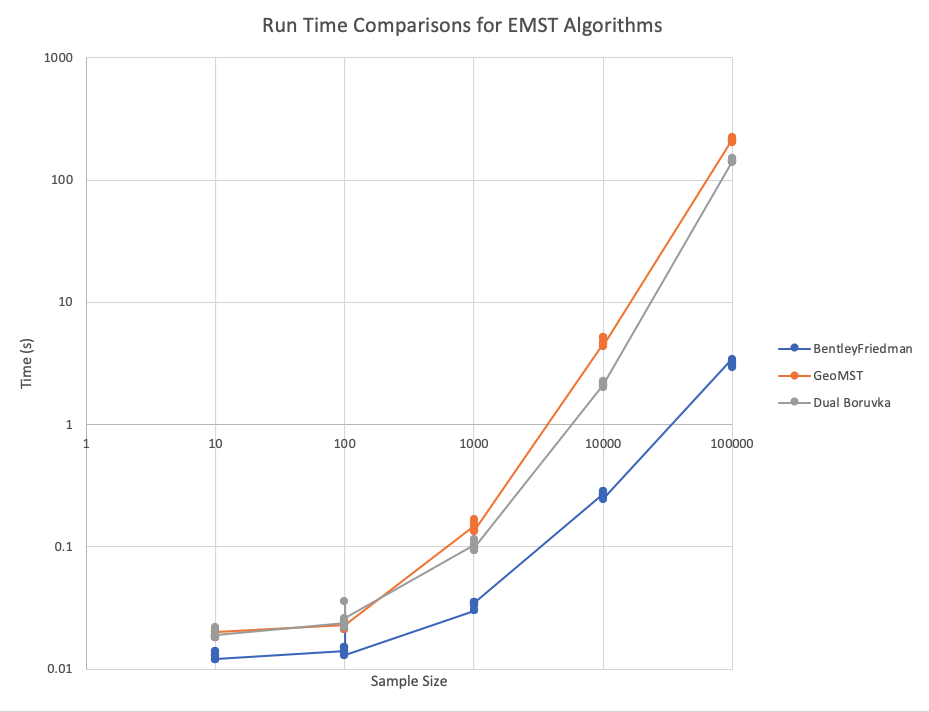
\includegraphics[width=\textwidth]{data.png}
	\end{center}
	\caption{Random points in a cube}
\end{figure}

We can also increases the dimensionality up to $d=20$ to see how such an increase affects these algorithms (Figure 2). When the dimensionality scales, Bentley Friedman's algorithm becomes more in-line with the other two in terms of runtime. This is to be expected since kd trees suffers an overhead cost that is exponential with respect to the dimension of the data.

\begin{figure}
	\begin{center}
		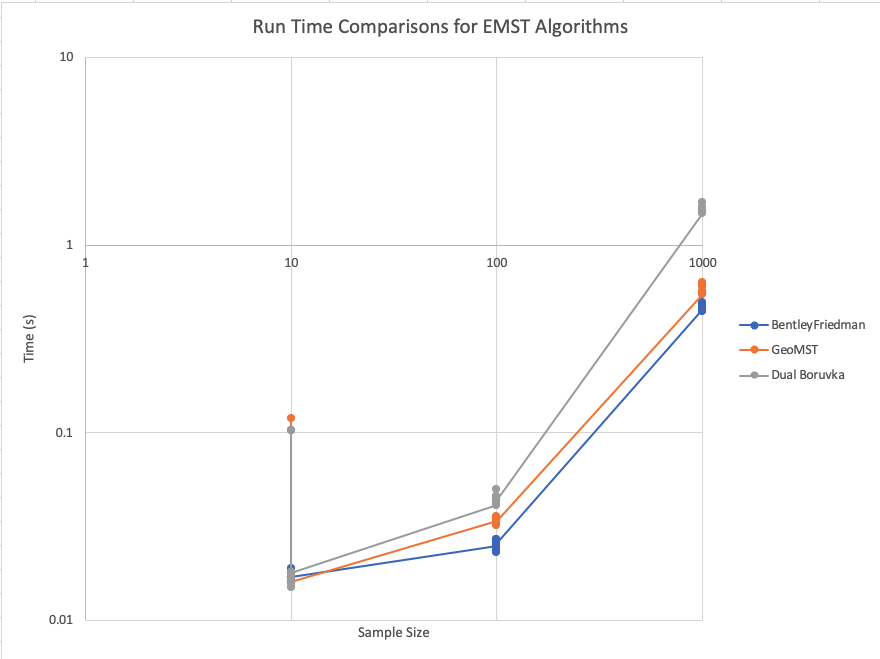
\includegraphics[width=\textwidth]{data2.png}
	\end{center}
	\caption{Random points in a cube}
\end{figure}

If readers wish to test our code on dimensions other than what we have, know that the only variable that determines the dimensional data is DIM in poly.cpp. 

\section{Conclusion}

While GeoMST and Dual Boruvka's algorithms are state of the art MST algorithms well suited for large computations, they are highly complex. If implemented without care, it can run significantly slower than simple Bentley Friedman due to the number of steps involved. In low dimensions, it is best to stick to Bentley Friedman, as kd tree has a $2^d$ overhead that remains insignificant if $d$ is small.    


\begin{thebibliography}{9}
	\bibitem{Friedman} J. Bentley and J. Friedman. Fast Algorithms forConstructing Minimal Spanning Trees in CoordinateSpaces.IEEE T. Comput., 27:97–105, 1978.
	\bibitem{Narasihman} Narasimhan, Giri \& Zachariasen, Martin. (2001). Geometric Minimum Spanning Trees via Well-Separated Pair Decompositions. ACM Journal of Experimental Algorithmics. 6. 6. 10.1145/945394.945400. 
	\bibitem{Dual} March, William \& Ram, Parikshit \& Gray, Alexander. (2010). Fast Euclidean Minimum Spanning Tree: Algorithm, analysis, and applications. Proceedings of the ACM SIGKDD International Conference on Knowledge Discovery and Data Mining. 603-612. 10.1145/1835804.1835882. 
	\bibitem{Callahan} Callahan, Paul. (1995). Dealing with higher dimensions [microform] : the well-separated pair decomposition and its applications /. 

\end{thebibliography}

\end{document}
